\documentclass[11pt]{article}
\usepackage[margin=1in]{geometry}
\usepackage{graphicx}
\usepackage{booktabs}
\usepackage{amsmath}
\usepackage{amssymb}
\usepackage{float}
\usepackage[T1]{fontenc}
\usepackage[colorlinks=true,allcolors=blue!60!black]{hyperref}
\usepackage{xcolor}
\usepackage{caption}
\captionsetup{font=small,labelfont=bf}
\newcommand{\ph}[1]{\texttt{#1}}
\newcommand{\tgeo}{\tau_{\mathrm{geo}}}

\title{\bf The Critical Core Radius: A Geometric Certificate for\\
Phone Separability in Frame-Level MFCC Space}
\author{}
\date{}

\begin{document}
\maketitle
\vspace{-2.5em}

\begin{abstract}
\noindent
Density-based clustering fails on frame-level MFCC features, and the failure is
usually reported without attribution: the same negative result is produced by a
poor algorithm choice, by poor hyperparameters, and by classes that genuinely
overlap. We separate these causes with a controlled ablation. For each phone we
fit a full-covariance Gaussian and draw Metropolis--Hastings samples restricted
to a Mahalanobis ball of radius $\tau$ around the class mean, which preserves
the class means and covariance orientations while making the amount of tail mass
a free parameter. Clustering quality then becomes a curve in $\tau$ rather than
a single verdict. We show that this curve is monotone --- every tightening step
improves NMI --- but that reading it naively is a trap: as $\tau \to 0$ the
sampler's acceptance rate collapses to zero, the chain freezes at the class
mean, and DBSCAN attains NMI $=1.0$ by clustering 39 point masses. We therefore
introduce a quantity that requires no clustering algorithm at all. For a pair of
classes, $\tau_{ij} = \min_x \max\big(d_M(x,\mu_i;\Sigma_i),
d_M(x,\mu_j;\Sigma_j)\big)$ is a convex program whose value is the largest
radius at which the two cores are provably disjoint. Its minimum over pairs is a
\emph{certificate}: below it, separability is guaranteed by geometry.
For the four acoustically distant classes \ph{aa}, \ph{n}, \ph{sh}, \ph{sil} the
certificate is $1.205\sigma$ and sits in a healthy sampling regime, so the
near-perfect clustering reported there is real. For all 39 phones the
certificate is $0.222\sigma$ --- inside the frozen regime, where acceptance is
$\le 0.002$. \textbf{No radius exists at which the 39 phone cores are
simultaneously provably separated and non-degenerate.} We validate the
certificate against an independent classifier: over all 741 phone pairs,
$\tau_{ij}$ predicts held-out confusion with Spearman $\rho = -0.849$
($p \approx 10^{-206}$), and 14 of the 20 tightest pairs are among the 20 most
confused. Per phone, accuracy is predicted not by the nearest competitor
($\rho = 0.13$, n.s.) but by \emph{crowding}, the mean of the ten smallest
$\tau_{ij}$ ($\rho = 0.80$, $p = 7 \times 10^{-10}$). Finally we release a 39-way
$K$-shot support set of Mahalanobis-ranked real frames with honest held-out
baselines: 39-way top-1 accuracy is $0.368$ against a chance rate of $0.026$.
\end{abstract}

\section{Introduction}

Clustering frame-level acoustic features is the most direct formulation of
unsupervised phone-unit discovery, and density-based methods such as DBSCAN are
a natural fit: they do not require the number of units in advance, and they
encode the intuition that a phone is a dense region of acoustic space. On MFCC
frames they do not work. Tuned aggressively they either label the majority of
frames as noise or collapse everything into one cluster.

That much is known. The difficulty is attribution. A negative clustering result
is compatible with at least three explanations --- the wrong algorithm, the
wrong hyperparameters, or a representation in which the classes are not
separable at all --- and reporting the failure does not distinguish them. This
paper is about distinguishing them.

Our instrument is a synthetic dataset that inherits its class geometry from the
real data but exposes the overlap as a knob. We fit one full-covariance Gaussian
$\mathcal{N}(\mu_k, \Sigma_k)$ per phone and sample from it truncated to
$\{x : d_M(x,\mu_k) \le \tau\}$. At large $\tau$ the sample reproduces the
overlap of the real data; as $\tau$ shrinks the classes contract toward their
means and the overlap is removed in a controlled way. Running an identical
clustering sweep at each $\tau$ converts a binary failure into a curve.

The curve alone, however, is not enough, and the reason is the main
methodological point of this paper. As $\tau \to 0$ every class contracts to a
point and any algorithm trivially succeeds, so a sufficiently small $\tau$
always ``works''. We make this concrete rather than treating it as a caveat:
the Metropolis--Hastings acceptance rate is a direct measure of whether the core
is still a distribution, and at $\tau \le 0.25\sigma$ with 39 classes it falls
to $0.002$ or below. The apparently perfect clustering in that regime is an
artifact of a frozen chain.

This motivates a quantity defined without reference to any clustering algorithm.
For two classes we ask for the smallest radius at which their cores touch,
\[
\tau_{ij} \;=\; \min_x\, \max\big( d_M(x,\mu_i;\Sigma_i),\;
d_M(x,\mu_j;\Sigma_j) \big),
\]
a convex program with a unique optimum. If $\tau < \tau_{ij}$ the two truncated
supports are disjoint sets, so the minimum of $\tau_{ij}$ over pairs is a
sufficient condition for separability that no algorithm can improve on. Our
contributions are:

\begin{enumerate}
\item \textbf{A tail-truncation ablation} attributing the failure of DBSCAN on
MFCC frames to class overlap rather than to the algorithm, and turning it into a
monotone curve in $\tau$ (\S\ref{sec:sweep}).
\item \textbf{An explicit degeneracy diagnostic.} The MH acceptance rate
identifies the regime in which apparent clustering success is an artifact,
which we show is exactly where the 39-class problem becomes separable
(\S\ref{sec:sweep}).
\item \textbf{The certificate $\tau_{ij}$} (\S\ref{sec:cert}), computed for all
741 phone pairs, together with its scaling in inventory size: the certificate
falls from $1.64\sigma$ at $K=2$ to $0.222\sigma$ at $K=39$.
\item \textbf{External validation} (\S\ref{sec:valid}): $\tau_{ij}$ predicts the
held-out confusions of an unrelated classifier at $\rho = -0.849$, and a
crowding statistic derived from it predicts per-phone accuracy at
$\rho = 0.80$.
\item \textbf{A released support set and honest baselines}
(\S\ref{sec:support}), including a correction to previously reported episode
accuracies that were measured with queries drawn from the support pool.
\end{enumerate}

\section{Related Work}

\textbf{Density-based clustering.} DBSCAN~\cite{ester1996} defines clusters as
regions of high density separated by regions of low density, with a global
radius $\varepsilon$ and a minimum neighbourhood count. Its known weakness is
data with variable density, which motivated OPTICS~\cite{ankerst1999} and
HDBSCAN~\cite{campello2013}; we evaluate all three.

\textbf{Acoustic unit discovery.} Unsupervised discovery of subword units has
been driven by the ZeroSpeech challenge series~\cite{versteegh2015}, with
Dirichlet-process mixture approaches~\cite{lee2012} among the strongest
frame-level clustering baselines. Our conclusion --- that the limiting factor is
the representation --- is consistent with the field's move toward learned
features.

\textbf{Learned speech representations.} wav2vec 2.0~\cite{baevski2020},
HuBERT~\cite{hsu2021} and WavLM~\cite{chen2022} produce representations whose
intermediate layers are substantially more phonetically linear than MFCCs.
Recomputing our certificate on those layers is the natural continuation
(\S\ref{sec:limits}).

\textbf{Few-shot classification.} Matching Networks~\cite{vinyals2016} and
Prototypical Networks~\cite{snell2017} learn embeddings in which
nearest-neighbour or nearest-centroid classification succeeds from a handful of
examples. The support set we release is in exactly the form these methods
consume.

\section{Data and Setup}

We use the TIMIT~\cite{garofolo1993} training partition: 4{,}620 utterances,
each stored as a $(T,12)$ matrix of MFCC frames with a frame-level phone
transcript of $(\text{label}, \text{start}, \text{end})$ triples in frame units.
Expanding the transcripts gives 1{,}419{,}678 labelled frames over the standard
39-symbol reduced inventory~\cite{leehon1989}, including \ph{sil}.

The frame distribution is severely skewed: \ph{sil} alone accounts for 367{,}150
frames (25.9\%) and the smallest class \ph{b} for 3{,}823. All experiments
therefore use a class-stratified subset --- 1{,}500 frames per phone at $K=39$,
3{,}000 at $K=4$ --- sampled without replacement. This is not a convenience: a
density method estimates one global density scale, and on unstratified counts
that scale is set by silence alone.

Features are standardized with a \texttt{StandardScaler} fit on the stratified
subset. Standardization is necessary because $c_0$ (log-energy) has a numeric
range roughly an order of magnitude larger than $c_1$--$c_{11}$, which carry most
of the phonetic contrast, while DBSCAN scores neighbourhoods with an unweighted
Euclidean metric. All runs use seed $0$.

\section{The Failure on Real Frames}
\label{sec:baseline}

We first establish that the failure is a property of the data rather than of one
algorithm. On a five-class subset (\ph{s}, \ph{ih}, \ph{aa}, \ph{iy}, \ph{n};
\ph{sil} excluded because it dominates)\footnote{An earlier internal report
describes this subset as the five densest non-silence classes, which would
substitute \ph{ae} for \ph{n}. The run that produced Table~\ref{tab:five} used
\ph{n}: its pool of 352{,}543 frames matches
$84{,}491 + 84{,}270 + 73{,}885 + 62{,}901 + 46{,}996$ exactly.}
on a balanced 10{,}000-frame sample, we swept DBSCAN over
$\varepsilon \in [1.6,2.4]$ and $\mathrm{min\_samples} \in \{5,8,10,15,20\}$
(45 configurations, with the $\varepsilon$ grid set from $k$-distance
quantiles), HDBSCAN over $\texttt{min\_cluster\_size} \in [30,1000]$, OPTICS
over $\xi \in [0.03,0.30]$, a 132-dimensional context-window variant ($\pm5$
frames, PCA-whitened to 30 components retaining 95\% variance), and a
5-component full-covariance GMM as a non-density reference.

\begin{table}[H]
\centering
\caption{Five-class comparison on 10{,}000 balanced frames. The best
density-based NMI covers 17\% of the data; the best NMI overall comes from a
model that is not density-based at all.}
\label{tab:five}
\begin{tabular}{llrrrr}
\toprule
Method & Parameters & Clusters & Coverage & NMI & ARI \\
\midrule
DBSCAN            & $\varepsilon=1.6$, $ms=8$ &  5 & 0.633 & 0.109 & 0.078 \\
DBSCAN            & $\varepsilon=1.4$, $ms=8$ & 11 & 0.351 & 0.163 & 0.108 \\
HDBSCAN           & $\mathit{mcs}=50$         &  2 & 0.166 & 0.233 & 0.069 \\
DBSCAN (132D ctx) & $\varepsilon=2.4$, $ms=8$ &  5 & 0.127 & 0.225 & 0.064 \\
OPTICS            & $ms=10$, $\xi$ sweep      &  0 & 0.000 & 0.000 & 0.000 \\
GMM               & 5 full-cov.\ components   &  5 & 1.000 & \textbf{0.555} & \textbf{0.525} \\
\bottomrule
\end{tabular}
\end{table}

Three readings set up the rest of the paper. The density-based family trades
coverage against purity and never obtains both: the context-window variant
reaches 0.978 clustered purity on 12.7\% of frames, and HDBSCAN's honest answer
is two clusters, one an almost perfectly pure \ph{s}. OPTICS finds no usable
reachability valleys at all, indicating that the density transitions are flat
rather than merely mis-thresholded --- visible directly in the $k$-distance
curves (Figure~\ref{fig:hist-raw}, right), which rise smoothly with no elbow.
And a GMM, which models each class as an overlapping ellipsoid instead of
thresholding a global density, roughly doubles the best density-based NMI at
full coverage. All three point at overlapping class supports.

\begin{figure}[H]
\centering
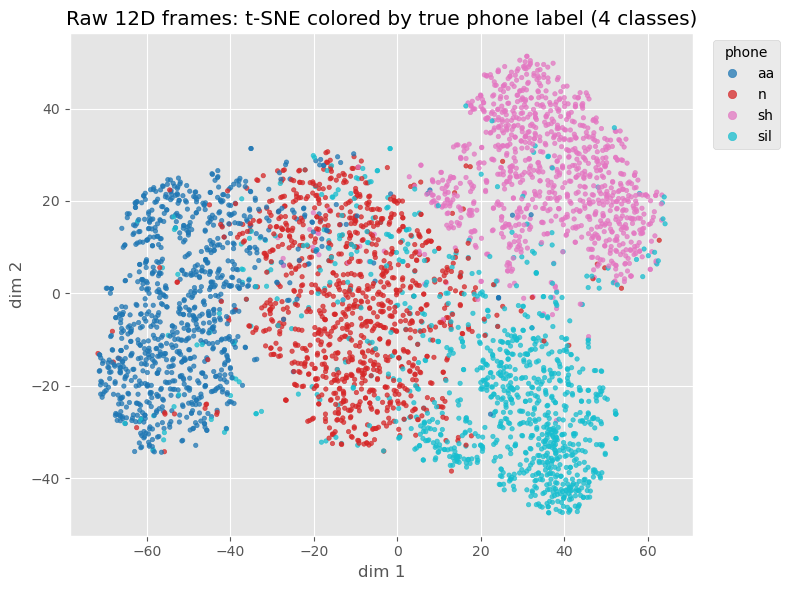
\includegraphics[width=0.46\textwidth]{assets/hist_raw_tsne_4class.png}
\hfill
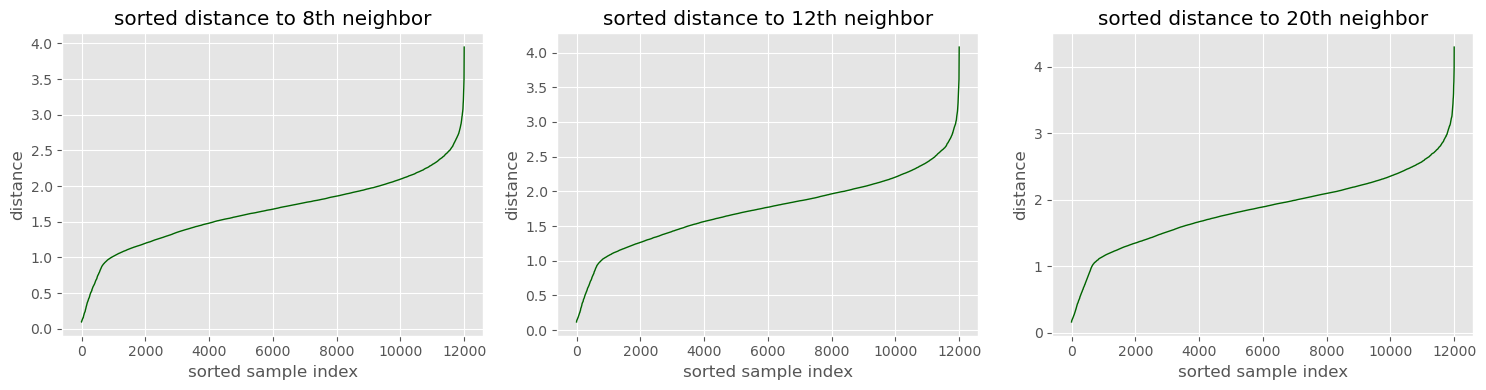
\includegraphics[width=0.52\textwidth]{assets/hist_kdistance_raw.png}
\caption{Left: t-SNE of 4{,}000 raw standardized frames from the four-class
subset, coloured by true phone. \ph{sh} forms a distinct cloud; \ph{aa},
\ph{n} and \ph{sil} overlap along their boundaries. Right: sorted distance to
the $k$-th nearest neighbour at $k = 8, 12, 20$. The absence of a sharp elbow is
why no single $\varepsilon$ works.}
\label{fig:hist-raw}
\end{figure}

\section{Method: Core Sampling}
\label{sec:method}

\subsection{Per-class Gaussians}

At $K=4$ we fit a four-component full-covariance GMM by EM with
\texttt{means\_init} set to the per-phone sample means and \texttt{weights\_init}
to the per-phone frequencies, then reorder components by nearest mean. The
recovered mapping is $\{\ph{aa}, \ph{n}, \ph{sh}, \ph{sil}\}$ with weights
$[0.256, 0.417, 0.247, 0.081]$, i.e.\ EM does keep each component bound to its
intended phone at this scale.

At $K=39$ this is no longer safe: joint EM over 39 components re-mixes them and
destroys the component-to-phone binding on which the whole diagnostic depends.
We therefore fit each Gaussian independently on its own class-conditioned
frames,
\[
\mu_k = \frac{1}{N_k}\!\!\sum_{i:y_i=k}\!\! x_i,
\qquad
\Sigma_k = \frac{1}{N_k-1}\!\!\sum_{i:y_i=k}\!\!(x_i-\mu_k)(x_i-\mu_k)^{\!\top}
+ \lambda I,
\]
with $\lambda = 10^{-4}$ as a numerical guard, which makes the binding hold by
construction.

\subsection{Truncated sampling}

For component $k$ we sample from
\[
\pi_k(x) \;\propto\; \mathcal{N}(x;\mu_k,\Sigma_k)\;
\mathbf{1}\!\left[d_M(x,\mu_k)\le\tau\right],
\qquad
d_M(x,\mu_k)=\sqrt{(x-\mu_k)^{\!\top}\Sigma_k^{-1}(x-\mu_k)},
\]
by Metropolis--Hastings with a symmetric Gaussian random-walk proposal
$x' = x + s\,\Sigma_k^{1/2}\eta$, $\eta\sim\mathcal{N}(0,I)$. Symmetry reduces
the acceptance ratio to
\[
\alpha(x\to x') = \min\!\Big(1,\;
\exp\!\big[-\tfrac{1}{2}\big(d_M^2(x',\mu_k)-d_M^2(x,\mu_k)\big)\big]\Big)\,
\mathbf{1}\!\left[d_M(x',\mu_k)\le\tau\right].
\]
We use burn-in 500, thinning 3, and $s = 0.25$ for $\tau \ge 1.2$, $s = 0.15$
below. The indicator is the entire point of the construction: it deletes the
tails, where adjacent phones meet, and leaves the means and covariance
orientations untouched.

\subsection{Selection rule}

At each $\tau$ we sweep $\varepsilon \in [0.10,1.00]$ in steps of $0.05$ and
$\mathrm{min\_samples} \in \{5,10\}$, and select the configuration maximizing NMI
subject to a noise budget of $0.4$. The noise budget is not optional. Ranking by
proximity to the target cluster count instead rewards a degenerate solution: at
$\tau=1.5$, $K=39$ that rule selects a run with 38 clusters of which one holds
4{,}860 points spanning 21 phones at 10\% purity, while 71\% of points are noise.

\section{The $\tau$ Sweep and the Degenerate Regime}
\label{sec:sweep}

\begin{table}[H]
\centering
\caption{DBSCAN on MCMC cores as a function of core radius $\tau$, 250 samples
per class, best configuration per row under the noise budget. NMI improves
monotonically as $\tau$ shrinks --- but so does the acceptance rate, and the top
rows are sampling a frozen chain rather than a distribution.}
\label{tab:sweep}
\begin{tabular}{rrrrrrrr}
\toprule
$\tau$ & MH accept. & $\varepsilon$ & $ms$ & Clusters & Noise & NMI & ARI \\
\midrule
0.15 & 0.000 & 0.15 & 5 &  39 & 0.000 & 1.000 & 1.000 \\
0.20 & 0.000 & 0.25 & 5 &  39 & 0.000 & 1.000 & 1.000 \\
0.25 & 0.002 & 0.35 & 5 &  39 & 0.000 & 1.000 & 1.000 \\
\midrule
0.30 & 0.006 & 0.35 & 10 &  44 & 0.001 & 0.985 & 0.951 \\
0.40 & 0.028 & 0.45 & 5 &  34 & 0.000 & 0.973 & 0.862 \\
0.50 & 0.075 & 0.40 & 5 &  52 & 0.007 & 0.951 & 0.825 \\
0.60 & 0.134 & 0.45 & 5 &  50 & 0.009 & 0.924 & 0.741 \\
0.75 & 0.232 & 0.50 & 5 &  54 & 0.026 & 0.780 & 0.325 \\
1.00 & 0.370 & 0.55 & 5 & 249 & 0.132 & 0.644 & 0.167 \\
1.25 & 0.227 & 0.65 & 5 & 368 & 0.258 & 0.551 & 0.090 \\
1.50 & 0.309 & 0.75 & 5 & 343 & 0.238 & 0.459 & 0.048 \\
\bottomrule
\end{tabular}
\end{table}

The monotone trend is unambiguous: every tightening of $\tau$ improves NMI, from
$0.459$ at $\tau=1.5$ to $1.000$ at $\tau \le 0.25$. Read alone, the table says
the classes are recoverable. The acceptance column says otherwise. At
$\tau \le 0.25$ the Metropolis chain accepts $0.2\%$ of proposals or fewer: it
never leaves its initial state at $\mu_k$, so the ``cluster'' for each phone is
250 copies of the class mean, and DBSCAN is separating 39 point masses. The
perfect scores in the top three rows measure nothing about the representation.

The same protocol on the four-class subset behaves completely differently.
There, NMI $= 1.000$ holds across $\tau \in [0.25, 1.75]$ with acceptance
between $0.08$ and $0.39$ --- a wide window in which the cores are genuine
distributions \emph{and} DBSCAN recovers them. This contrast, shown in
Figure~\ref{fig:regimes}, is the substantive result: the four-class success is
real and the 39-class success is not.

\begin{figure}[H]
\centering
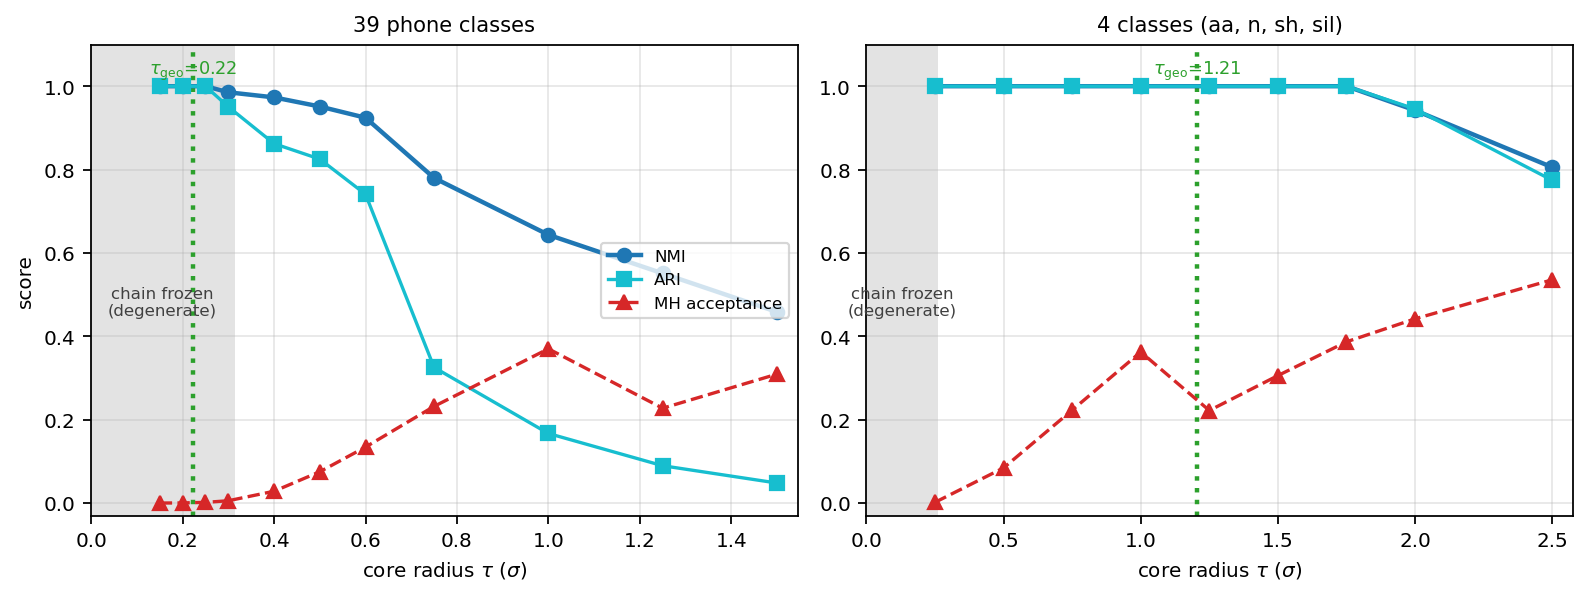
\includegraphics[width=\textwidth]{assets/fig_tau_regimes.png}
\caption{Clustering quality and MH acceptance rate against core radius $\tau$.
Shaded: the regime where acceptance $< 0.02$ and the sampler has frozen at the
class mean. Dotted green: the geometric certificate $\tgeo$ of
\S\ref{sec:cert}. \emph{Left,} 39 classes --- the certificate lies inside the
frozen region, so there is no radius that is both certified and non-degenerate.
\emph{Right,} four classes --- the certificate lies well outside it, and a wide
valid window exists.}
\label{fig:regimes}
\end{figure}

\begin{figure}[H]
\centering
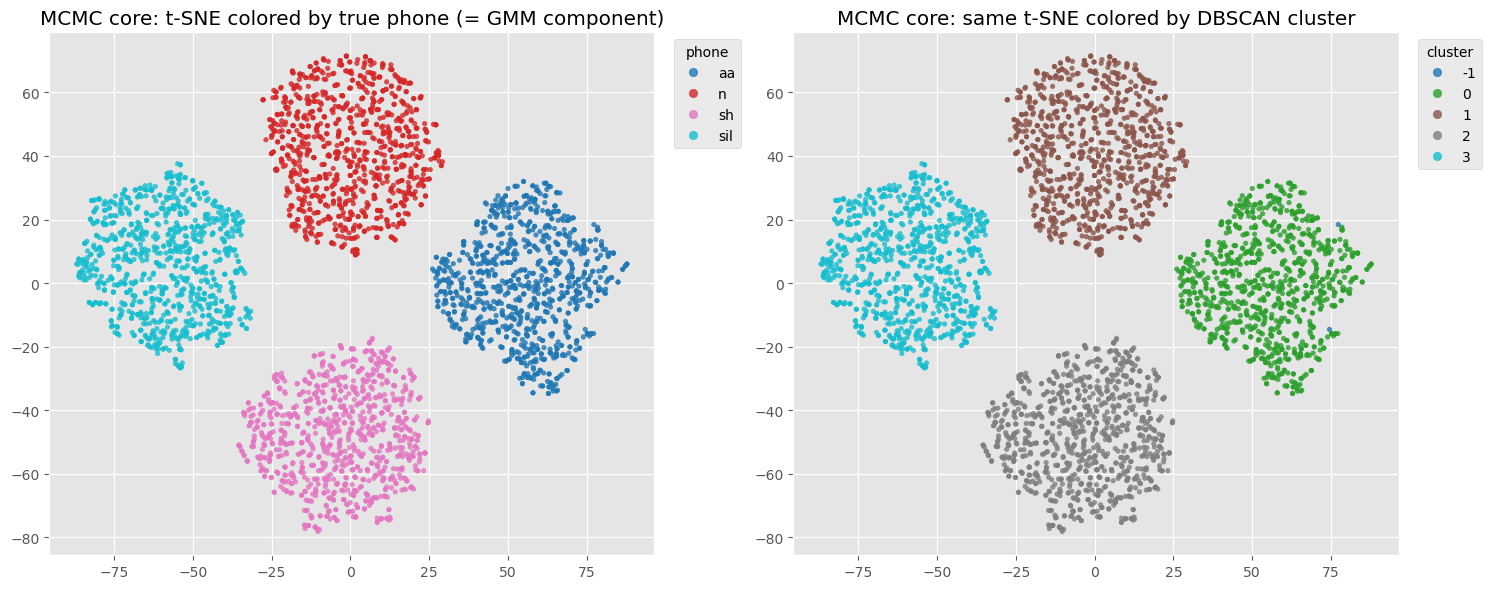
\includegraphics[width=0.49\textwidth]{assets/hist_core_vs_dbscan_4class.png}
\hfill
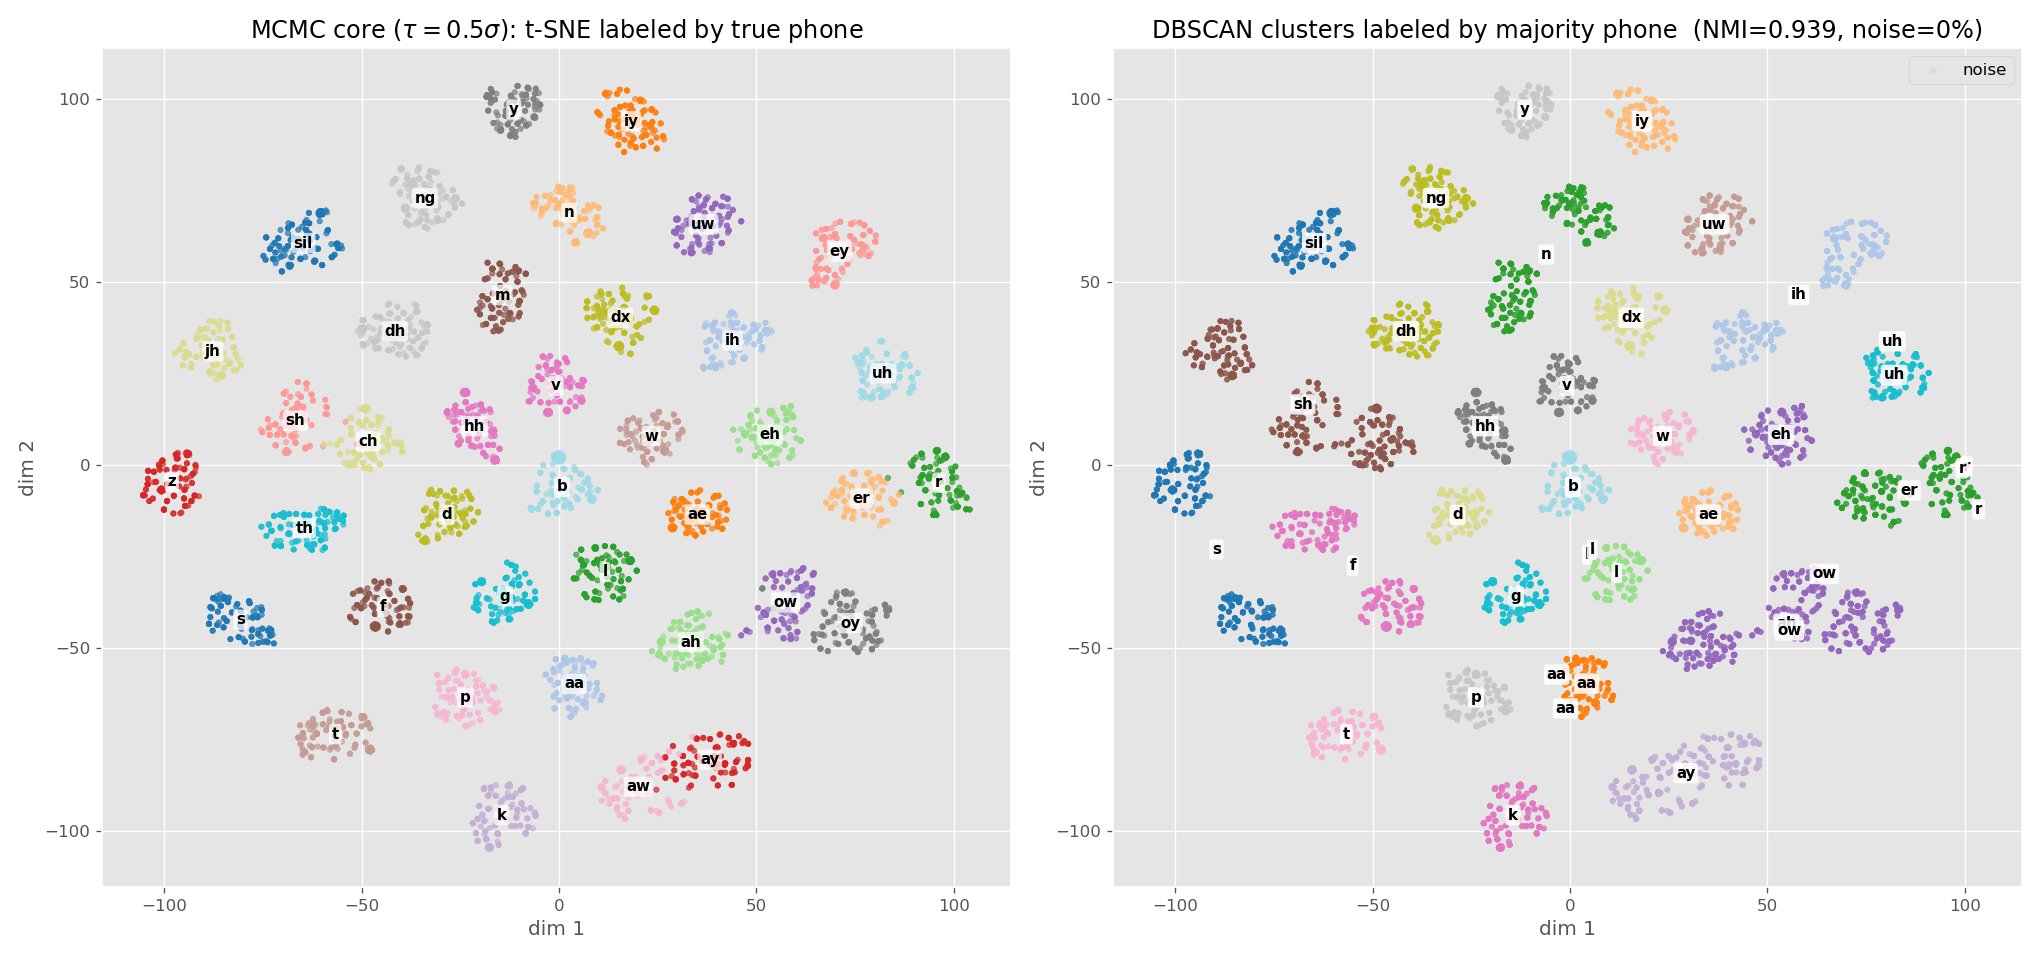
\includegraphics[width=0.49\textwidth]{assets/hist_labeled_clusters_39.png}
\caption{Left: four-class cores at $\tau=1.5$, truth versus DBSCAN --- the
panels are visually identical. Right: 39-class cores at $\tau=0.5$, with each
cluster annotated by its majority phone. The cluster count is close to target
but the map is not bijective: adjacent blobs share cluster identities.}
\label{fig:tsne}
\end{figure}

\paragraph{Relation to a previously reported result.} An earlier run of this
experiment (400--500 samples per class, coarser $\varepsilon$ grid, ranking that
also rewarded proximity to 39 clusters) reported exactly 39 clusters at
$\tau=0.5$ with NMI $=0.939$ and noise $0.0018$, and was summarized as a
recovery of the inventory. The re-run in Table~\ref{tab:sweep} reaches a similar
NMI ($0.951$) at the same $\tau$ but finds 52 clusters, and the earlier run's own
composition analysis had already shown that only 31 of 39 phones were the
majority of any cluster, with 8 phones (\ph{ih}, \ph{ay}, \ph{z}, \ph{sh},
\ph{m}, \ph{oy}, \ph{jh}, \ph{th}) absorbed into neighbours. The exact cluster
count is therefore sensitive to the sweep grid and to the selection rule, and
should not be read as recovery of the inventory. The monotone $\tau$ trend is
robust across both runs; the cluster count is not.

\section{A Geometric Certificate}
\label{sec:cert}

The acceptance-rate diagnostic tells us when a $\tau$ is degenerate, but it is
still tied to a sampler and a clustering algorithm. We now remove both.

\subsection{Definition}

For classes $i$ and $j$ define
\begin{equation}
\tau_{ij} \;=\; \min_{x \in \mathbb{R}^{12}}\;
\max\big(d_M(x,\mu_i;\Sigma_i),\; d_M(x,\mu_j;\Sigma_j)\big).
\label{eq:cert}
\end{equation}
Each $d_M(\cdot,\mu_k;\Sigma_k)$ is a norm of an affine function of $x$ and
therefore convex; the pointwise maximum of convex functions is convex; so
(\ref{eq:cert}) is a convex program with a unique optimal value, solved here in
its epigraph form $\min t$ s.t.\ $d_M(x,\mu_i) \le t$, $d_M(x,\mu_j)\le t$ by
SLSQP with analytic gradients.

The interpretation is immediate. The truncated supports
$B_i(\tau) = \{x : d_M(x,\mu_i) \le \tau\}$ and $B_j(\tau)$ intersect if and
only if there exists $x$ with both distances $\le \tau$, i.e.\ iff
$\tau \ge \tau_{ij}$. Hence for $\tau < \tau_{ij}$ the two cores are disjoint
sets, and
\[
\tgeo \;=\; \min_{i \ne j} \tau_{ij}
\]
is a radius below which \emph{all} class cores are pairwise disjoint. This is a
statement about the class geometry alone: no clustering algorithm, no sampler,
no hyperparameter.

Note the direction of the guarantee. $\tau < \tgeo$ is sufficient for disjoint
supports, not necessary for a clustering method to succeed --- with finite
samples the region near the touching point is very sparsely populated, so
DBSCAN can and does succeed at $\tau$ somewhat above $\tgeo$. The certificate is
a conservative bound, and both empirical windows respect it.

\subsection{Results}

\begin{table}[H]
\centering
\caption{The ten least-separable phone pairs by certificate, with the Euclidean
distance between class means for comparison. Phones marked $\dagger$ are those
absorbed by DBSCAN in the 39-class run.}
\label{tab:pairs}
\begin{tabular}{lrr@{\qquad}lrr}
\toprule
Pair & $\tau_{ij}$ & $\|\mu_i-\mu_j\|$ & Pair & $\tau_{ij}$ & $\|\mu_i-\mu_j\|$ \\
\midrule
\ph{ay}$\dagger$/\ph{aw} & 0.222 & 0.496 & \ph{ch}/\ph{jh}$\dagger$  & 0.416 & 0.595 \\
\ph{sh}$\dagger$/\ph{ch} & 0.258 & 0.348 & \ph{ih}$\dagger$/\ph{ey}  & 0.442 & 0.874 \\
\ph{er}/\ph{r}           & 0.307 & 0.514 & \ph{ah}/\ph{ow}           & 0.445 & 0.983 \\
\ph{ow}/\ph{oy}$\dagger$ & 0.322 & 0.479 & \ph{n}/\ph{m}$\dagger$    & 0.479 & 0.764 \\
\ph{sh}$\dagger$/\ph{jh}$\dagger$ & 0.379 & 0.516 & \ph{aa}/\ph{aw}  & 0.486 & 1.096 \\
\bottomrule
\end{tabular}
\end{table}

For the full inventory $\tgeo = 0.222\sigma$, set by \ph{ay}/\ph{aw}. For the
four-class subset $\tgeo = 1.205\sigma$, set by \ph{n}/\ph{sil}. Placing these
on Figure~\ref{fig:regimes} gives the paper's central claim:

\begin{quote}
\textbf{At $K=39$ the certificate ($0.222\sigma$) lies inside the frozen regime
(acceptance $\le 0.002$). Certified separability and non-degenerate sampling
have no common radius. At $K=4$ the certificate ($1.205\sigma$) lies in a
healthy regime (acceptance $0.36$ at $\tau=1.0$), and the observed recovery is
genuine.}
\end{quote}

The certificate is correlated with the distance between class means
($r = 0.887$) but is not a rescaling of it, and the disagreements are
informative. By mean distance the hardest pair is \ph{sh}/\ph{ch} ($0.348$);
by certificate it is \ph{ay}/\ph{aw}, whose means are $42\%$ further apart
($0.496$) but whose covariances are oriented so that the ellipsoids reach toward
each other. Diphthongs are exactly the classes for which a frame-level Gaussian
is widest, and the certificate accounts for that where a mean distance cannot.

\begin{figure}[H]
\centering
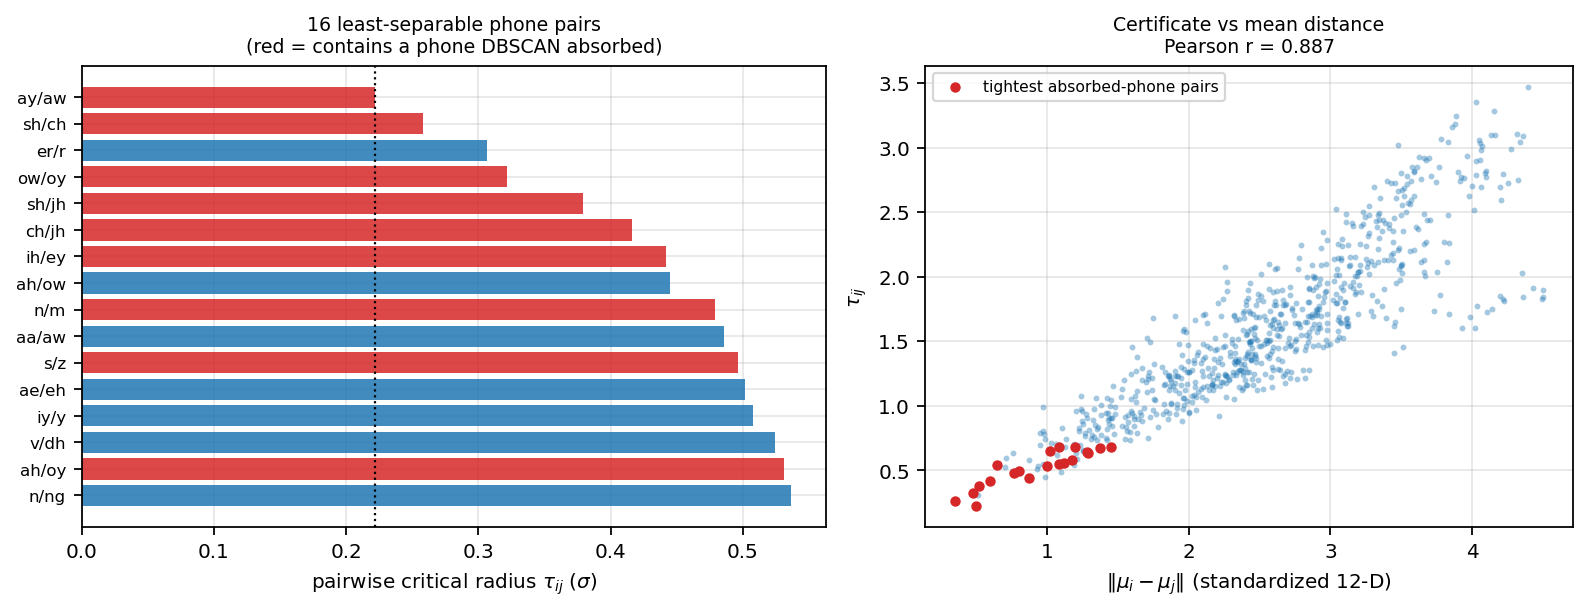
\includegraphics[width=\textwidth]{assets/fig_pairs.png}
\caption{Left: the 16 least-separable pairs; red bars contain a phone that
DBSCAN absorbed. Right: certificate against distance between class means over
all 741 pairs.}
\label{fig:pairs}
\end{figure}

\subsection{Scaling with inventory size}

Because $\tau_{ij}$ is defined per pair, $\tgeo$ for any subset of classes is a
minimum over a submatrix, and the scaling of separability with inventory size
can be computed exactly without re-running anything. Averaging over 400 random
subsets per size:

\begin{table}[H]
\centering
\caption{$\tgeo$ against inventory size $K$, mean $\pm$ sd over random subsets.}
\begin{tabular}{lrrrrrrrr}
\toprule
$K$ & 2 & 4 & 8 & 12 & 16 & 24 & 32 & 39 \\
\midrule
$\tgeo$ & $1.64 \pm .60$ & $0.88 \pm .27$ & $0.54 \pm .16$ & $0.42 \pm .13$
& $0.35 \pm .10$ & $0.29 \pm .07$ & $0.24 \pm .03$ & $0.222$ \\
\bottomrule
\end{tabular}
\end{table}

Separability decays steeply and then saturates: by $K \approx 24$ the certificate
is essentially pinned by the single worst pair present in almost every subset.
The four-class set actually used (\ph{aa}, \ph{n}, \ph{sh}, \ph{sil},
$\tgeo = 1.205$) sits near the 90th percentile of random four-class subsets
(p90 $= 1.234$) --- it was chosen for acoustic distinctness, and it is
quantifiably an easy case. Any conclusion drawn from four hand-picked classes
therefore does not transfer to the full inventory, which is precisely what the
39-class experiment found the hard way.

\begin{figure}[H]
\centering
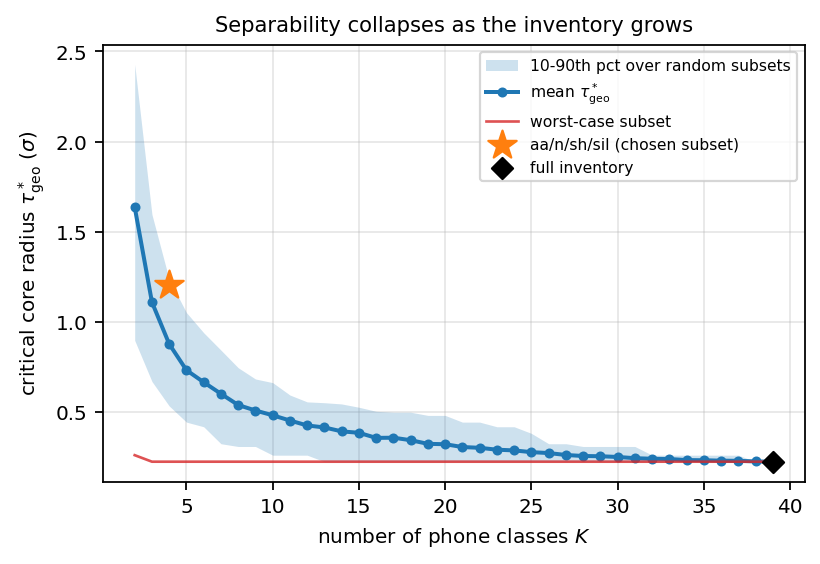
\includegraphics[width=0.62\textwidth]{assets/fig_tau_vs_K.png}
\caption{Certificate against inventory size. The chosen four-class subset
(star) is near the top decile of its size; the full inventory (diamond) is set
by \ph{ay}/\ph{aw}.}
\label{fig:tauK}
\end{figure}

\section{Validating the Certificate}
\label{sec:valid}

A geometric quantity is only useful if it predicts behaviour that was not used
to construct it. We test it against a classifier that shares no machinery with
DBSCAN: quadratic discriminant analysis on \emph{held-out real frames}
(\S\ref{sec:support}), for which we compute the symmetric confusion rate
$S_{ij}$ between every pair of phones.

\begin{itemize}
\item Over all \textbf{741 pairs}, $\tau_{ij}$ predicts $S_{ij}$ with Spearman
$\rho = -0.849$ ($p \approx 1.5\times10^{-206}$); restricted to the 581 pairs
ever confused, $\rho = -0.803$.
\item \textbf{14 of the 20} pairs with the smallest certificate are among the 20
most-confused pairs.
\item The most-confused pairs are \ph{sh}/\ph{ch} (certificate rank 1 of 741),
\ph{s}/\ph{z} (rank 10), \ph{er}/\ph{r} (rank 2), \ph{iy}/\ph{y} (rank 12) and
\ph{sh}/\ph{jh} (rank 4).
\end{itemize}

\paragraph{Per-phone accuracy needs crowding, not the nearest neighbour.} Our
first hypothesis --- that a phone's accuracy is governed by its closest
competitor, $\min_j \tau_{ij}$ --- \textbf{fails}: $\rho = 0.126$, $p = 0.44$.
Aggregating over the neighbourhood succeeds. The mean of a phone's ten smallest
$\tau_{ij}$ predicts its held-out accuracy at $\rho = 0.804$
($p = 6.8\times10^{-10}$), and $\sum_j \tau_{ij}^{-1}$ performs comparably
($\rho = 0.802$). A phone is hard when it sits in a crowded neighbourhood, not
when it has one close rival --- which is consistent with a 39-way decision in
which every competitor can claim probability mass.

\begin{figure}[H]
\centering
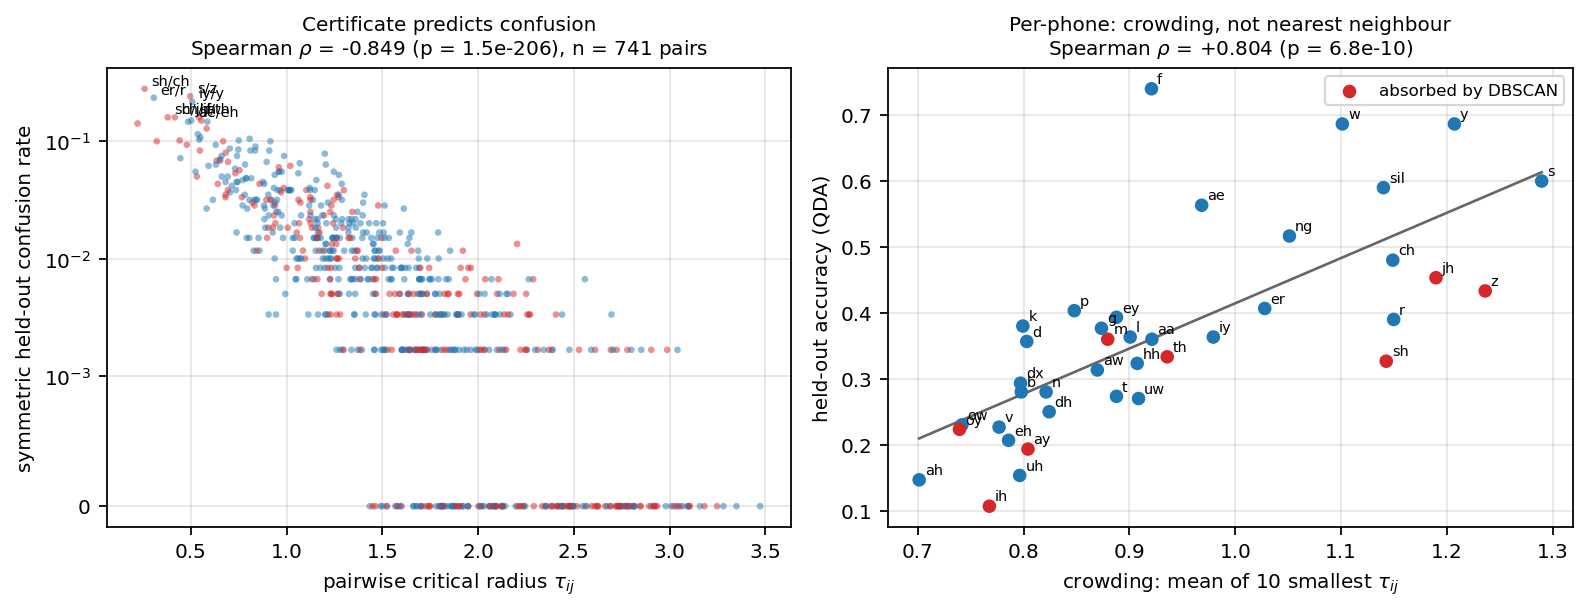
\includegraphics[width=\textwidth]{assets/fig_certificate_validation.png}
\caption{Left: certificate against symmetric held-out confusion for all 741
pairs (log-scaled ordinate; red points involve a DBSCAN-absorbed phone).
Right: per-phone accuracy against crowding.}
\label{fig:valid}
\end{figure}

\section{Support Set and Held-Out Baselines}
\label{sec:support}

The per-class Gaussians also support a constructive use. For each phone we score
every real frame in the stratified subset by $d_M(x_i,\mu_k)$ and keep the
$K=10$ smallest: the most prototypical real exemplars, equivalently the $K$
frames of highest density under the class component. This yields a 39-way
10-shot support set of 390 real frames, each traceable to its source
$(\textit{utt\_id},\textit{frame\_idx})$.

The construction uses only each phone's own $(\mu_k,\Sigma_k)$ and never a
pairwise comparison, so it stays well defined for the phones that clustering
cannot separate; discriminating those is precisely the task handed to a
downstream embedding. Per-phone prototype spread is itself interpretable:
\ph{sil} ($d_M \in [0.86,1.08]$), \ph{p}, \ph{v} and \ph{f} have the tightest
cores, while \ph{oy} ($[1.76,2.04]$), \ph{aw}, \ph{r} and \ph{ow} are widest ---
the diphthongs and rhotics again.

\subsection{Held-out evaluation}

We remove the 390 prototype frames from the corpus and sample 300 held-out
frames per phone (11{,}700 total), standardized with the stored scaler.

\begin{table}[H]
\centering
\caption{Held-out 39-way top-1 accuracy, 11{,}700 frames, no learned parameters.}
\label{tab:heldout}
\begin{tabular}{lr}
\toprule
Classifier & Accuracy \\
\midrule
Nearest prototype mean (Euclidean)              & 0.277 \\
Nearest class mean (Euclidean)                  & 0.297 \\
Minimum Mahalanobis to class Gaussian           & 0.335 \\
Gaussian log-likelihood, full covariance (QDA)  & \textbf{0.368} \\
\midrule
Chance                                          & 0.026 \\
\bottomrule
\end{tabular}
\end{table}

Three points. Accuracy is $14\times$ chance yet only $0.368$, which is the
quantitative version of this paper's thesis: a single 12-dimensional MFCC frame
carries real but limited phone identity. The ordering matters --- using the full
covariance (QDA) beats using only the mean by 7 points, so the class \emph{shape}
carries information that any centroid method discards, and this is exactly the
regime where a learned metric should help. And the eight phones DBSCAN absorbed
average $0.304$ against $0.384$ for the other 31, so the clustering diagnostic
and the supervised classifier agree on which phones are hard.

\begin{figure}[H]
\centering
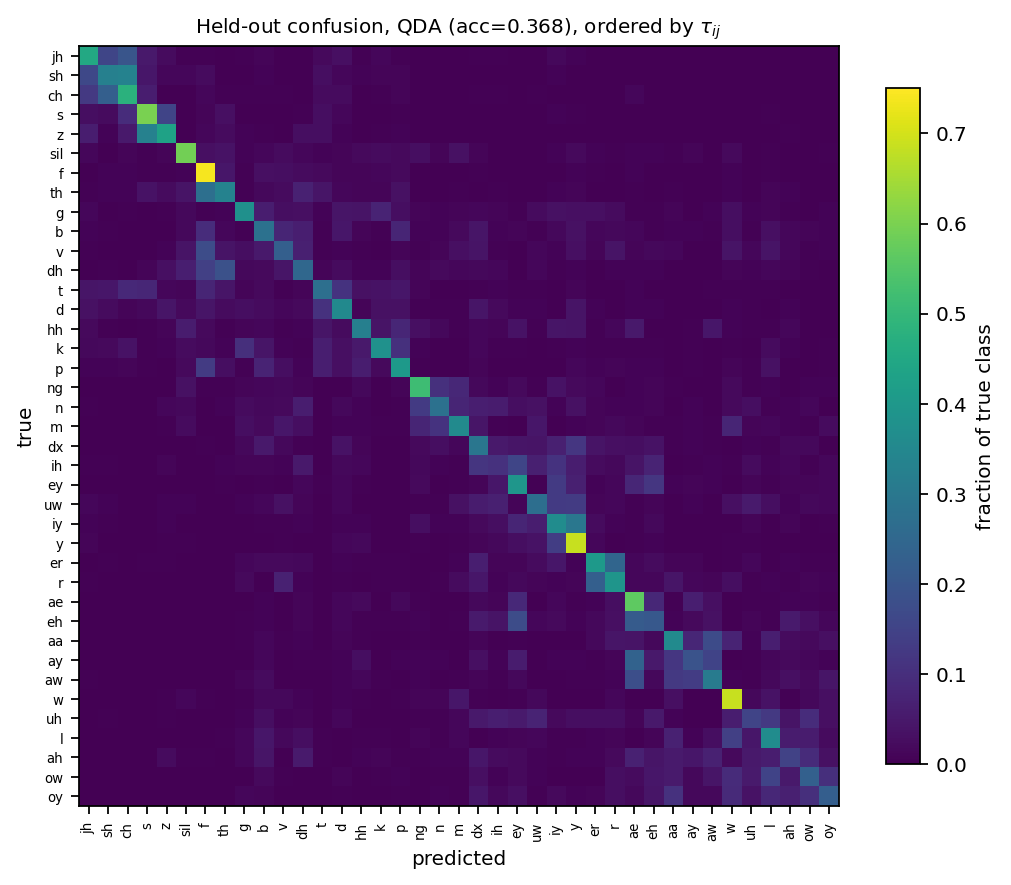
\includegraphics[width=0.66\textwidth]{assets/fig_heldout_confusion.png}
\caption{Held-out confusion for the QDA classifier, rows and columns ordered by
hierarchical clustering of the certificate matrix. Off-diagonal mass
concentrates in the blocks the certificate identifies.}
\label{fig:conf}
\end{figure}

\subsection{A correction to previously reported few-shot numbers}

Episode accuracies we reported previously drew query frames from the same pool
of 390 prototypes as the supports. Since every prototype is by construction
close to its class mean, this inflates accuracy substantially. Repeating the
protocol with queries drawn from held-out frames:

\begin{table}[H]
\centering
\caption{$N$-way $K$-shot nearest-centroid accuracy over 400 episodes. ``Pool''
draws queries from the prototype set (as previously reported); ``held-out''
draws them from unseen frames.}
\label{tab:kshot}
\begin{tabular}{lrrrr}
\toprule
& \multicolumn{2}{c}{1-shot} & \multicolumn{2}{c}{5-shot} \\
\cmidrule(lr){2-3}\cmidrule(lr){4-5}
$N$-way & pool & held-out & pool & held-out \\
\midrule
5   & 0.807 & 0.589 & 0.907 & 0.673 \\
10  & 0.693 & 0.442 & 0.816 & 0.521 \\
20  & 0.547 & 0.317 & 0.705 & 0.379 \\
39  & ---   & 0.207 & ---   & 0.262 \\
\bottomrule
\end{tabular}
\end{table}

The gap is 0.20--0.23 absolute throughout. The held-out column is the number a
learned few-shot model should be compared against; the pool column should not be
used.

\begin{figure}[H]
\centering
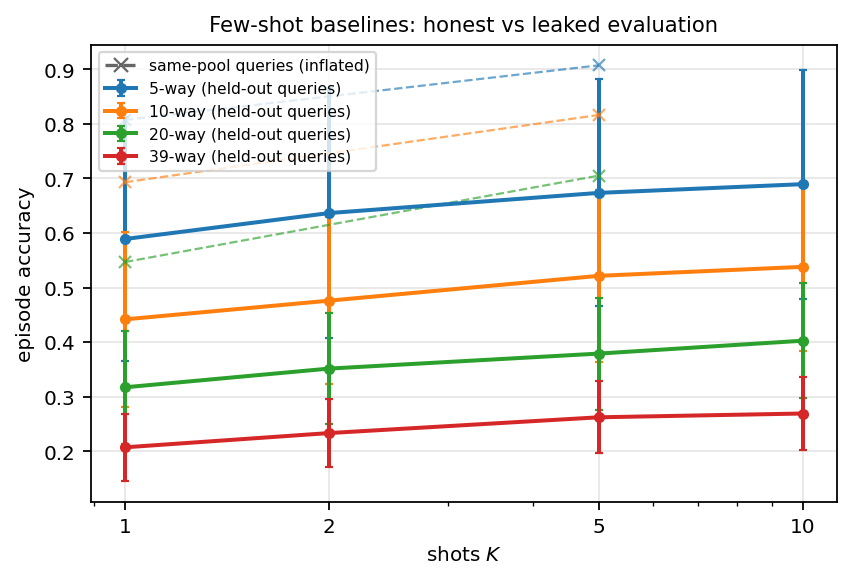
\includegraphics[width=0.58\textwidth]{assets/fig_kshot.png}
\caption{Few-shot baselines. Solid: held-out queries. Dashed: same-pool queries,
inflated by roughly 0.2 absolute at every setting.}
\label{fig:kshot}
\end{figure}

\section{Limitations}
\label{sec:limits}

\textbf{Gaussianity.} The certificate is exact for the truncated Gaussians it is
defined on, and only as good as that model is for real phones. Phones with
allophonic variation are plausibly multimodal, in which case a single ellipsoid
overstates their extent. A per-phone mixture, with the certificate taken as a
minimum over component pairs, is the natural generalization.

\textbf{One feature space.} Every claim here concerns 12-dimensional MFCCs. The
obvious control --- recomputing $\tau_{ij}$ on self-supervised representations,
where we expect a far larger certificate and where the crowding statistic
becomes a layer-selection criterion --- is not run here and is the single most
valuable next experiment.

\textbf{Frame-level only.} A frame is treated as i.i.d.\ and the trajectory
structure of a phone is discarded. The one context experiment we ran ($\pm5$
frames, 132D, PCA-whitened) raised clustered purity to 0.978 at 12.7\% coverage,
which is suggestive but not conclusive.

\textbf{Cluster counts are grid-sensitive.} As \S\ref{sec:sweep} documents, the
exact number of clusters recovered depends on the sweep grid and selection rule;
only the monotone trend and the certificate are stable.

\textbf{Single corpus.} TIMIT is read English, and the 39-symbol inventory
already merges some contrasts.

\section{Conclusion}

Density-based clustering of frame-level MFCCs fails for a reason that can be
measured rather than asserted. Replacing real frames with samples from per-class
Gaussians truncated at a controllable Mahalanobis radius turns the failure into
a monotone curve; the sampler's acceptance rate then reveals that the regime in
which the 39-class problem appears solved is one in which the cores have
collapsed to points. Removing the algorithm entirely, the convex program
(\ref{eq:cert}) gives a certificate of separability that depends only on the
class geometry: $1.205\sigma$ for four acoustically distant phones, and
$0.222\sigma$ for the full inventory --- the latter inside the degenerate
regime, so that no valid operating point exists. The certificate is not a
formal curiosity: it predicts the pairwise confusions of an unrelated
held-out classifier at $\rho = -0.849$, and an aggregate of it predicts
per-phone accuracy at $\rho = 0.80$. Together with a released 39-way $K$-shot
support set and corrected baselines, this converts a negative clustering result
into a measurement instrument for the learned representations that the result
says are necessary.

\section*{Reproducibility}

Artifacts: \texttt{dbscan\_variants\_5phone.ipynb} (Table~\ref{tab:five});
\texttt{dbscan\_4phone\_classes\_dim12.ipynb} and
\texttt{dbscan\_4phone\_mcmc\_gmm\_dim12.ipynb} (four-class);
\texttt{dbscan\_40phone\_mcmc\_gmm\_dim12.ipynb} (39-class, support set);
\texttt{use\_support\_set\_40phone.ipynb} (episodes); and
\texttt{support\_set\_40phone.pkl}, which bundles the 39 class Gaussians, the
scaler, the 390 prototypes with source metadata, and the DBSCAN configuration.
The certificate, the re-run $\tau$ sweep, the held-out evaluation and all
figures in \S\ref{sec:sweep}--\ref{sec:support} are produced by four standalone
scripts operating on the pickle and the corpus. Seed $0$ throughout.

\begin{thebibliography}{99}
\small
\bibitem{ester1996} M.~Ester, H.-P. Kriegel, J.~Sander, X.~Xu.
A density-based algorithm for discovering clusters in large spatial databases
with noise. \emph{KDD}, 1996.
\bibitem{ankerst1999} M.~Ankerst, M.~Breunig, H.-P. Kriegel, J.~Sander.
OPTICS: Ordering points to identify the clustering structure.
\emph{SIGMOD}, 1999.
\bibitem{campello2013} R.~Campello, D.~Moulavi, J.~Sander.
Density-based clustering based on hierarchical density estimates.
\emph{PAKDD}, 2013.
\bibitem{versteegh2015} M.~Versteegh et al.
The Zero Resource Speech Challenge 2015. \emph{Interspeech}, 2015.
\bibitem{lee2012} C.-Y. Lee, J.~Glass.
A nonparametric Bayesian approach to acoustic model discovery. \emph{ACL}, 2012.
\bibitem{baevski2020} A.~Baevski, Y.~Zhou, A.~Mohamed, M.~Auli.
wav2vec 2.0: A framework for self-supervised learning of speech
representations. \emph{NeurIPS}, 2020.
\bibitem{hsu2021} W.-N. Hsu et al.
HuBERT: Self-supervised speech representation learning by masked prediction of
hidden units. \emph{IEEE/ACM TASLP}, 2021.
\bibitem{chen2022} S.~Chen et al.
WavLM: Large-scale self-supervised pre-training for full stack speech
processing. \emph{IEEE JSTSP}, 2022.
\bibitem{vinyals2016} O.~Vinyals, C.~Blundell, T.~Lillicrap, K.~Kavukcuoglu,
D.~Wierstra. Matching networks for one shot learning. \emph{NeurIPS}, 2016.
\bibitem{snell2017} J.~Snell, K.~Swersky, R.~Zemel.
Prototypical networks for few-shot learning. \emph{NeurIPS}, 2017.
\bibitem{garofolo1993} J.~Garofolo et al.
TIMIT acoustic-phonetic continuous speech corpus. LDC, 1993.
\bibitem{leehon1989} K.-F. Lee, H.-W. Hon.
Speaker-independent phone recognition using hidden Markov models.
\emph{IEEE Trans.\ ASSP}, 1989.
\end{thebibliography}

\end{document}
